\section{Modèles}\label{sec: conception-database-models}
\subsection{Diagramme de classes}\label{subsec:conception-class-diagram}
\begin{figure}[ht]
    \centering
    \caption{Diagramme de classes}
    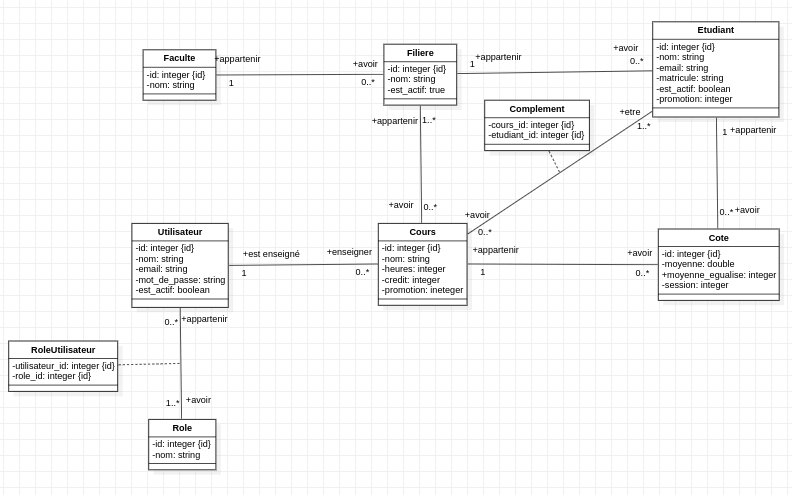
\includegraphics[width=1\linewidth]{class-diagram}
    \label{fig:class-diagram}
\end{figure}
\pagebreak

\subsection{Diagramme d'objets}\label{subsec:conception-object-diagram}
\begin{figure}[ht]
    \centering
    \caption{Diagramme d'objets}
    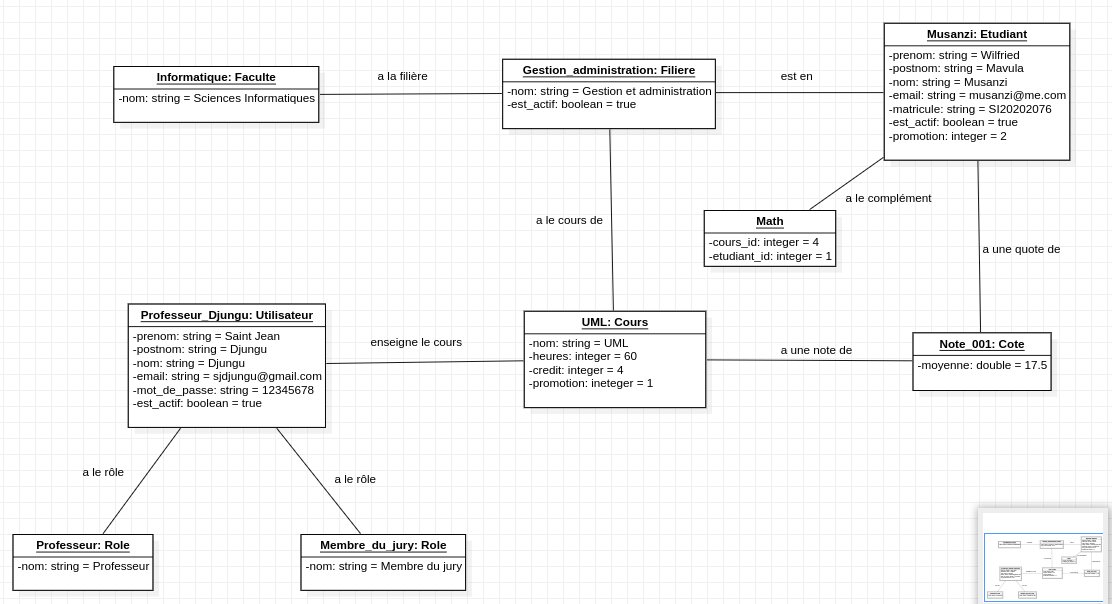
\includegraphics[width=1\linewidth]{object-diagram}
    \label{fig:object-diagram}
\end{figure}
\pagebreak


\subsection{Diagramme de cas d'utilisation}\label{subsec:conception-use-case-diagram}
\begin{figure}[ht]
    \caption{Cas d'utilisation : Gestion des ressources}
    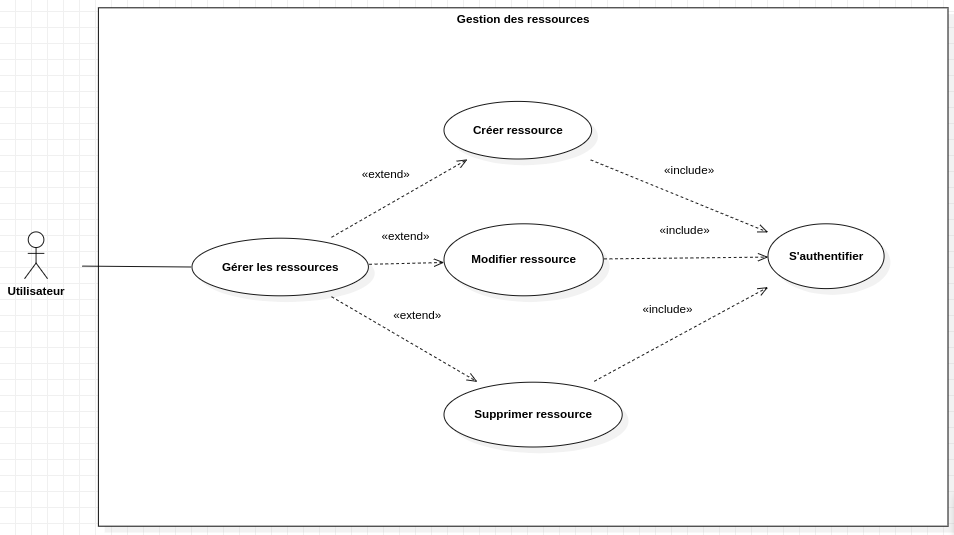
\includegraphics[width=1\linewidth]{use-cases/use-case}
    \centering
    \label{fig:ress-management}
\end{figure}

\begin{figure}[ht]
    \caption{Cas d'utilisation : Création des PDFs(Relevés)}
    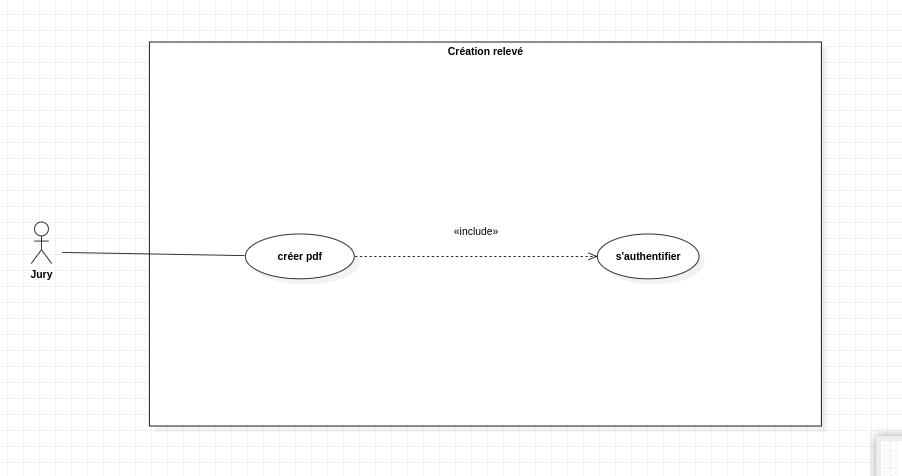
\includegraphics[width=1\linewidth]{use-cases/create-pdf}
    \centering
    \label{fig:create-pdf}
\end{figure}
\pagebreak

\begin{figure}[ht]
    \caption{Cas d'utilisation : Envoyer le pdf par mail}
    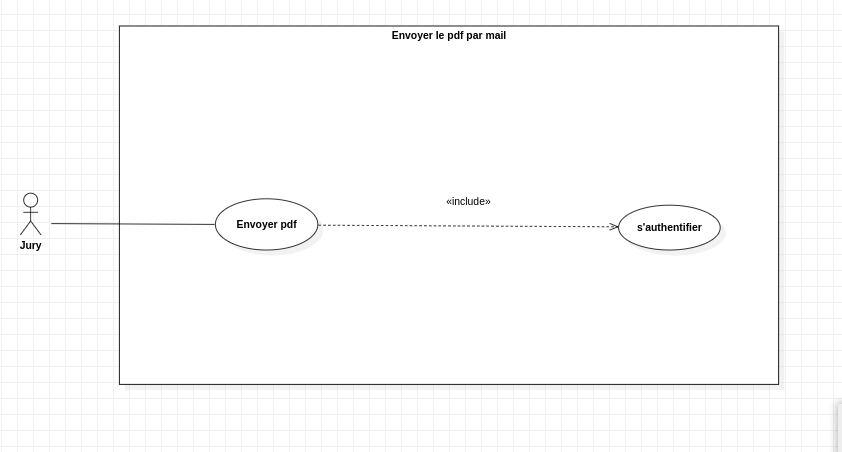
\includegraphics[width=1\linewidth]{use-cases/send-pdf}
    \centering
    \label{fig:send-pdf}
\end{figure}
\pagebreak

\subsection{Diagramme de séquence}\label{subsec:conception-sequence-diagram}
\begin{figure}[ht]
    \centering
    \caption{Diagramme de séquence}
    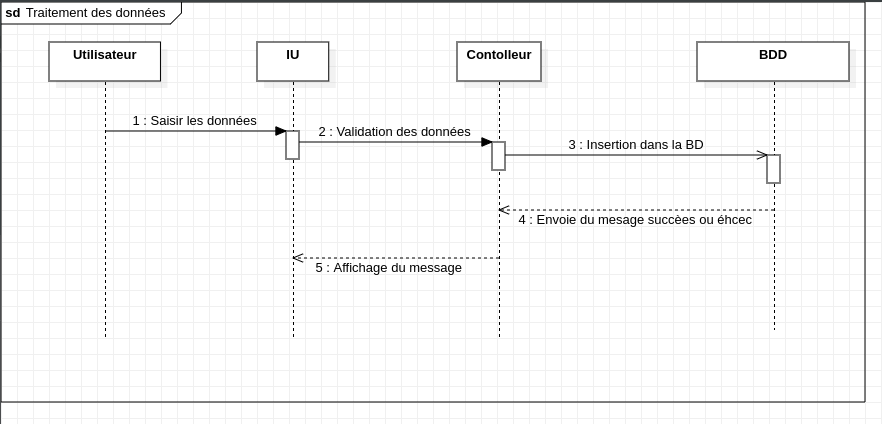
\includegraphics[width=1\linewidth]{sequence}
    \label{fig:sequence-diagram}
\end{figure}
\pagebreak